%
% $RCSfile$
%
% Copyright (c) 2005-2006. Christian Heller. All rights reserved.
%
% Permission is granted to copy, distribute and/or modify this document
% under the terms of the GNU Free Documentation License, Version 1.1 or
% any later version published by the Free Software Foundation; with no
% Invariant Sections, with no Front-Cover Texts and with no Back-Cover
% Texts. A copy of the license is included in the section entitled
% "GNU Free Documentation License".
%
% http://www.cybop.net
% - Cybernetics Oriented Programming -
%
% http://www.resmedicinae.org
% - Information in Medicine -
%
% Version: $Revision$ $Date$ $Author$
% Authors: Christian Heller <christian.heller@tuxtax.de>
%

\subsubsection{Overall Placement}
\label{overall_placement_heading}

Considering an overall computer system architecture, \emph{CYBOI} is situated
between the application knowledge existing in form of \emph{CYBOL} templates
and the \emph{Hardware} controlled by an \emph{Operating System} (OS) (figure
\ref{connection_figure}). CYBOI can thus also be called a
\emph{Knowledge-Hardware-Interface} (synonymous with \emph{Mind-Brain-Interface}).

\begin{figure}[ht]
    \begin{center}
        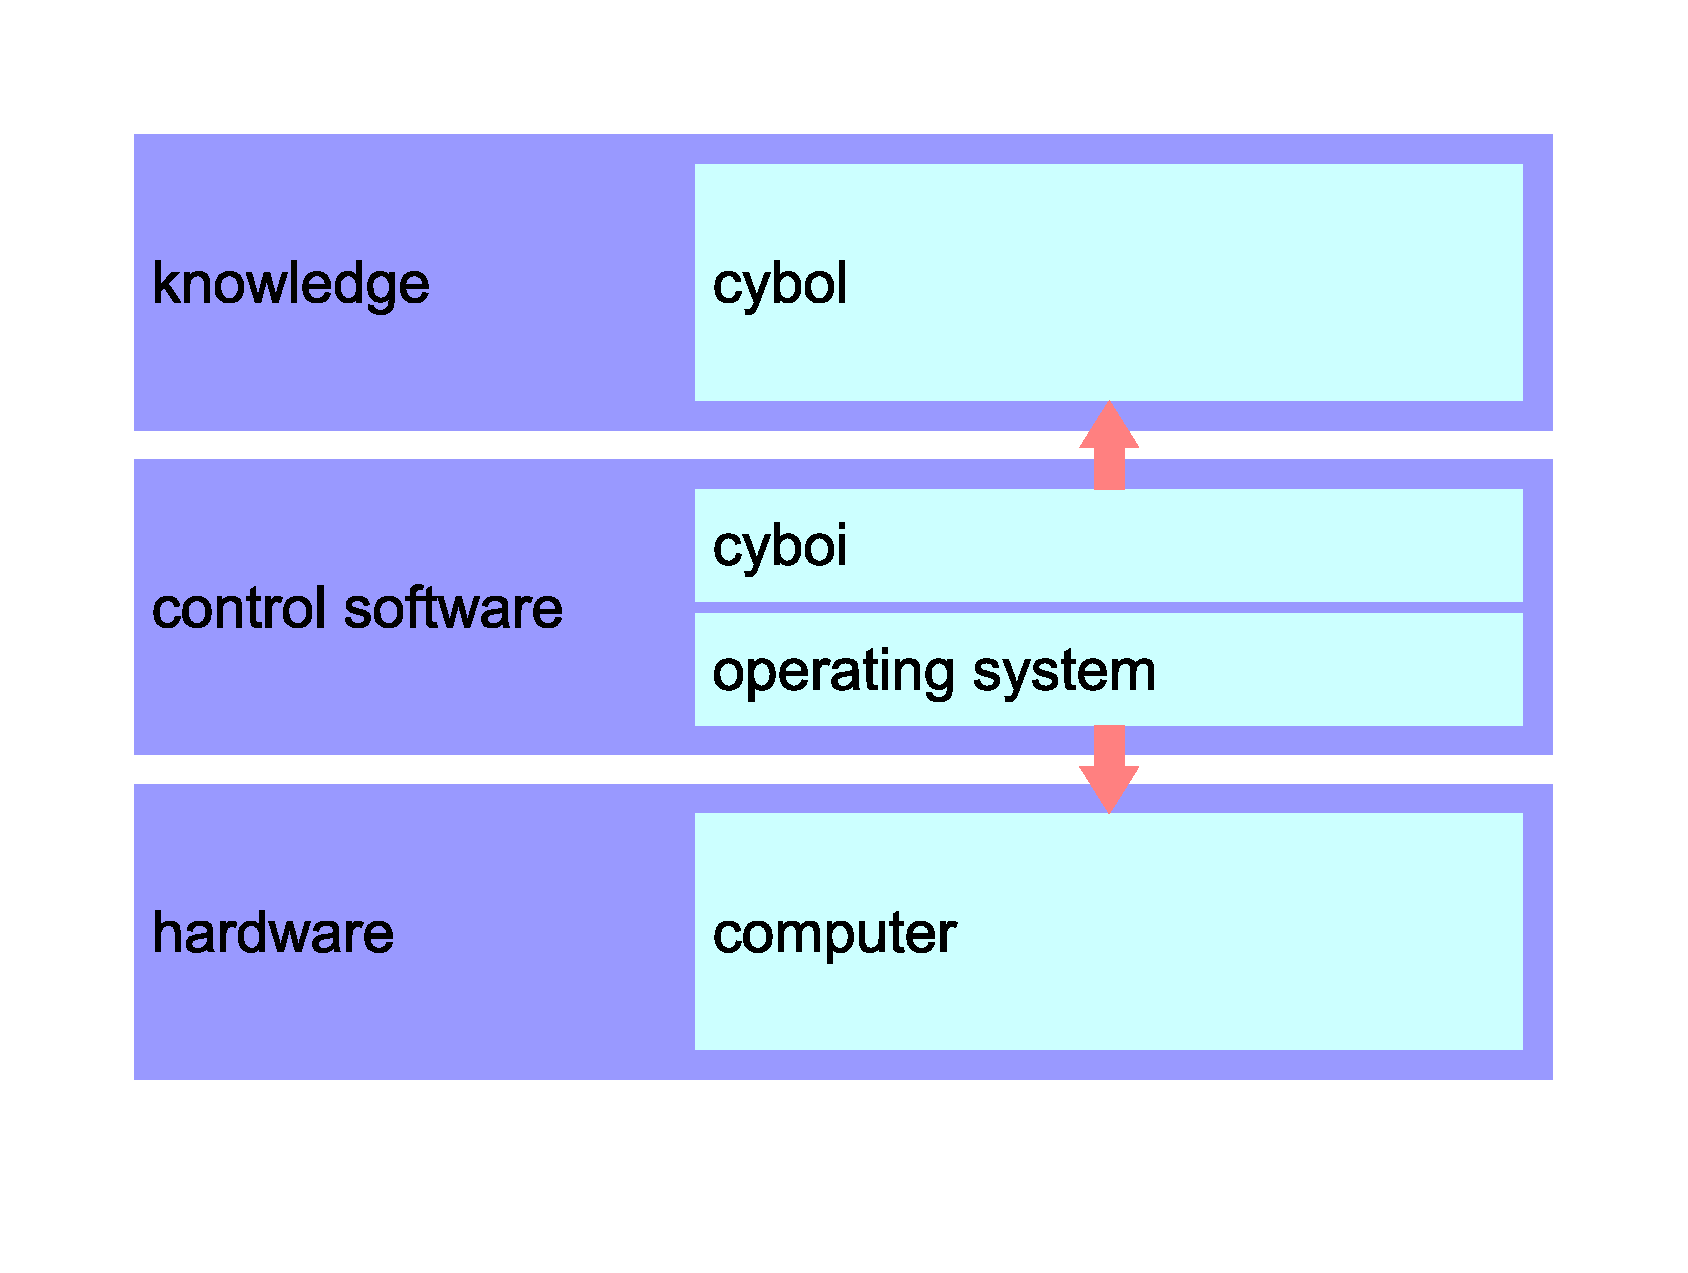
\includegraphics[scale=0.2]{vector/connection.eps}
        \caption{Knowledge -- Hardware Link}
        \label{connection_figure}
    \end{center}
\end{figure}

\begin{table}[ht]
    \begin{center}
        \begin{footnotesize}
        \begin{tabular}{| p{18mm} | p{18mm} | p{18mm} |}
            \hline
            \textbf{Criterion} & \textbf{Java World} & \textbf{CYBOP World}\\
            \hline
            Theory & OOP in Java & CYBOP\\
            \hline
            Language & Java & CYBOL\\
            \hline
            Interpreter & Java VM & CYBOI\\
            \hline
        \end{tabular}
        \end{footnotesize}
        \caption{Java-/ CYBOP World Analogies}
        \label{analogies_table}
    \end{center}
\end{table}

There are analogies to other systems run by language interpretation. Table
\ref{analogies_table} shows those between the \emph{Java-} and \emph{CYBOP}
world. Both are based on a programming theory, have a language and interpreter.
A theoretical model of a computer hardware- or -software system may be called
an \emph{Abstract Computer} or \emph{Abstract Machine} \cite{wikipedia}. If
being implemented as software simulation, or if containing an interpreter, it
is called a \emph{Virtual Machine} (VM). Kernighan and Pike write in their book
\emph{Practice of Programming} \cite{kernighan1999}:

\begin{quote}
� � Virtual machines are a wonderful, old idea, that latterly, through Java and
    the \emph{Java Virtual Machine} (JVM), came into fashion again. They are a
    simple possibility to gain portable and efficient program code, which can
    be written in a higher programming language.
\end{quote}

In that sense, CYBOI is certainly a VM. It provides low-level, platform-dependent
system functionality, close to the OS, together with a unified knowledge schema
(section \ref{knowledge_schema_heading}) which allows CYBOL applications to be
truly portable, well extensible and easier to program, because developers need
to concentrate on domain knowledge only. Since CYBOI interprets CYBOL sources
\emph{live} at system runtime, without the need for previous compilation (as in
Java), changes to CYBOL sources get into effect right away, without restarting
the system.
